%==================================================================
%==================================================================
\section{A null model}
\frame{\frametitle{Outline} \tableofcontents[currentsection]}
%==================================================================
\frame{\frametitle{Need for a null model}

  \paragraph{Motif counts} obviously depend on 
  \begin{itemize}
    \setlength{\itemsep}{1.15\baselineskip}
    \item the \emphase{size} of the network: $n \times m$
    \item the \emphase{density} of the network
    \item the \emphase{imbalance} between bottom-node degrees (specialist vs generalist pollinators)
    \item the \emphase{imbalance} between top-node degrees (specialist vs generalist plants)
  \end{itemize}
  
  \bigskip \bigskip \pause
  \paragraph{Bipartite expected degree distribution (\BEDD) model:} (in words)
  \begin{itemize}
    \setlength{\itemsep}{1.15\baselineskip}
    \item Consider $m$ pollinators ($i = 1, \dots m$): \\
    each plant $i$ has a specific propensity to interact (degree of generalism)
    \item Consider $n$ plants ($j = 1, \dots n$): \\
    each plant $j$ has a specific propensity to interact  (idem)
    \item The probability for pollinator $i$ and plant $j$ to interact is proportional to the product of their respective propensities.
  \end{itemize}

}

%==================================================================
\frame{\frametitle{\BEDD model}

  \paragraph{Bipartite expected degree distribution (\BEDD) model:} (formaly) \\~
  \begin{itemize}
    \setlength{\itemsep}{1.15\baselineskip}
    \item $\rho =$ network density
    \item $g =$ top node degree imbalance ($\int g = 1$)
    \item $h =$ bottom node degree imbalance ($\int h = 1$)
  \end{itemize}
  
  $$
  \{U_i\}_{i = 1, \dots m} \text{ iid } \sim \Ucal[0, 1] 
  \qquad \qquad 
  \{V_j\}_{j = 1, \dots n} \text{ iid } \sim \Ucal[0, 1]
  $$
  
  $$
  \Pbb\{i \sim j \mid U_i, V_j\} = \emphase{\rho \; g(U_i) \; h(V_j)}
  $$ 

  \bigskip
  (Bipartite version of the EDD model \refer{ChL02})
  
  \bigskip \bigskip \pause
  \paragraph{Model parameters:}
  $$
  \theta = (\rho, g, h).
  $$

}

%==================================================================
\frame{\frametitle{\BEDD model}

  \begin{tabular}{cccc}
    & & $h_0(v) =$ & $h(v) =$ \\
    \multicolumn{2}{c}{
      $\begin{array}{rl}
        \Pbb\{i \sim j \mid U_i, V_j\} & = \rho \; g(U_i) \; h(V_j) \\ \\
        \Esp (D_i \mid U_i) & = n \; \rho \; g(U_i) \\ \\
        \Esp (D_j \mid V_j) & = m \; \rho \; g(V_i) 
      \end{array}$
    } &
    \begin{tabular}{c} 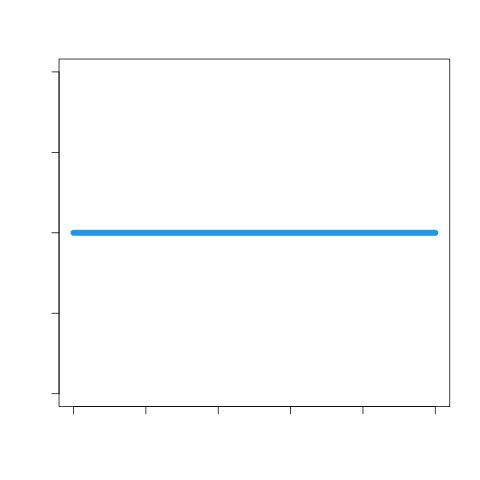
\includegraphics[width=.18\textwidth]{\fignet/FigMotifsBEDD-dist-h10} \end{tabular} &
    \begin{tabular}{c} 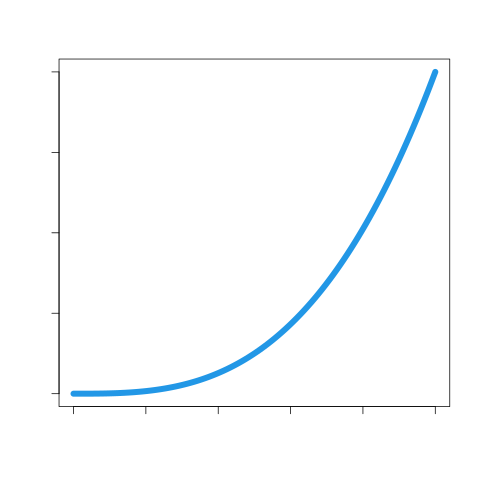
\includegraphics[width=.18\textwidth]{\fignet/FigMotifsBEDD-dist-h40} \end{tabular} \\
    \begin{tabular}{c} $g_0(u) =$ \end{tabular} &
    \begin{tabular}{c} 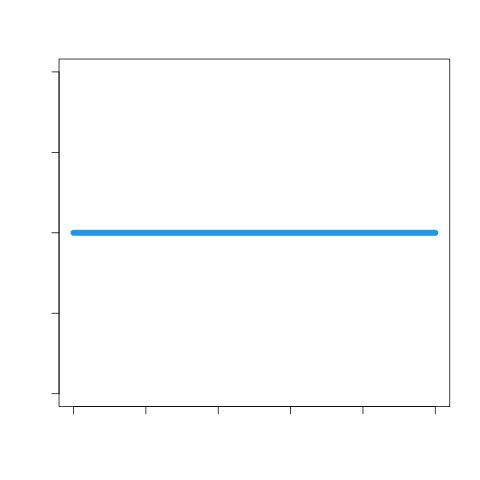
\includegraphics[width=.18\textwidth]{\fignet/FigMotifsBEDD-dist-g10} \end{tabular} &
    \begin{tabular}{c} 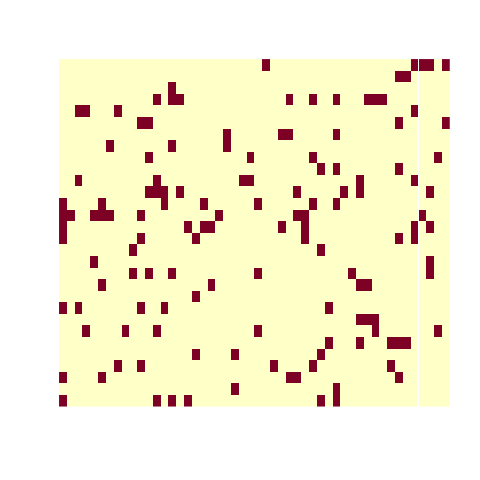
\includegraphics[width=.18\textwidth]{\fignet/FigMotifsBEDD-adj-g10-h10} \end{tabular} &
    \begin{tabular}{c} 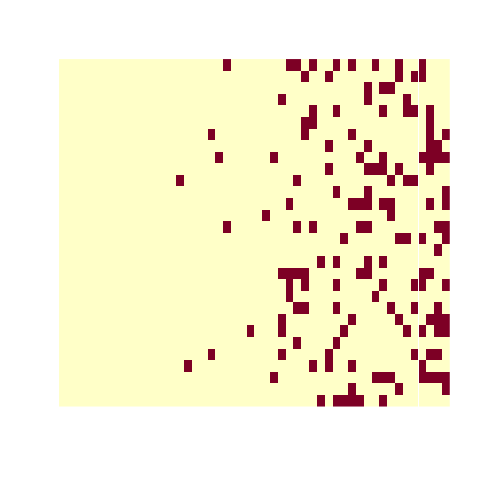
\includegraphics[width=.18\textwidth]{\fignet/FigMotifsBEDD-adj-g10-h40} \end{tabular} \\
    \begin{tabular}{c} $g(u) =$ \end{tabular} &
    \begin{tabular}{c} 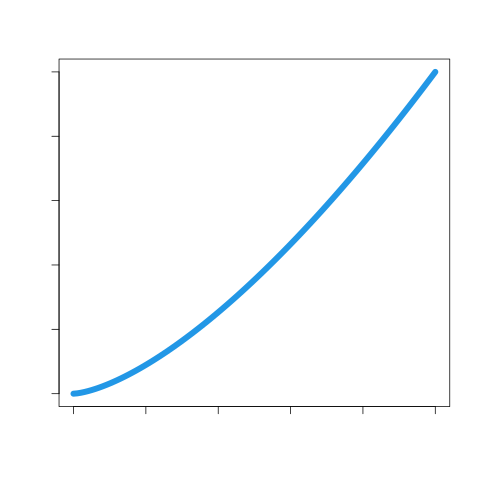
\includegraphics[width=.18\textwidth]{\fignet/FigMotifsBEDD-dist-g25} \end{tabular} &
    \begin{tabular}{c} 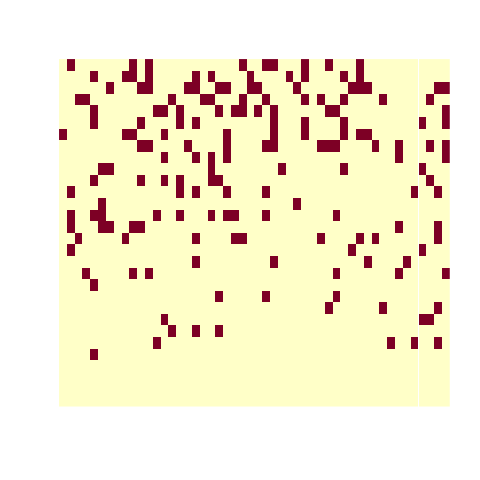
\includegraphics[width=.18\textwidth]{\fignet/FigMotifsBEDD-adj-g25-h10} \end{tabular} &
    \begin{tabular}{c} 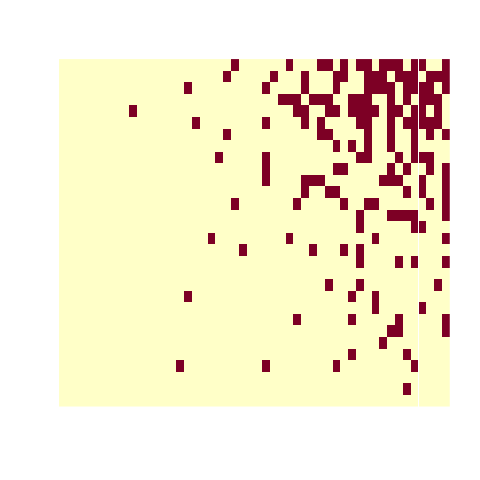
\includegraphics[width=.18\textwidth]{\fignet/FigMotifsBEDD-adj-g25-h40} \end{tabular} \\
  \end{tabular}
  
}

%==================================================================
\frame{\frametitle{Properties of the \BEDD model}

  \paragraph{Assumptions.}
  \begin{itemize}
    \setlength{\itemsep}{1\baselineskip}
    \item No preferred or avoided specific connexion
    \item \emphase{Graph-exchangeable} model: pollinators can be permuted and plants can be permuted
  \end{itemize}
  
  \bigskip \bigskip \pause
  \paragraph{Properties.}
  \begin{itemize}
    \setlength{\itemsep}{1\baselineskip}
    \item Expected degree for pollinator $i$ given $U_i$ : $n \; \rho \; g(U_i)$.
    \item Expected degree for plant $j$ given $V_j$ : $m \; \rho \; h(V_j)$.
    \item 'Nested' structure by construction
  \end{itemize}
  
  \bigskip \bigskip \pause
  \paragraph{Sufficient statistics} to fit \BEDD: 
  \begin{itemize}
    \setlength{\itemsep}{1\baselineskip}
    \item Pollinator degrees + plant degrees
    \item or, equivalently, star (single edge, top, bottom) frequencies
  \end{itemize}

  }

